

In our research group we have explored the synthesis of Gd-doped BaZrO$_3$ by a chemical synthesis method with guidance from Prof. Sergey Vyazovkin and Dr. Benjamin Yancey from the UAB Department of Chemistry. Technical assistance in implementing this synthesis procedure and in analyzing the resulting material was provided by high school student Ms. Graziella Camata \cite{GCamata2015}. Barium nitrate, zirconium tetraisopropoxide, citric acid, and ethylene glycol were employed in this synthesis, with the addition of gadolinium nitrate as the dopant source. A procedure based on the literature was cautiously followed to generate a BaZrO$_3$ powder nominally doped with Gd. The details of the approach are provided in this appendix. 

The basis of this synthesis depends on the use of precursor salts which are mixed through the formation of a polymer \cite{Bernardi2007, Rosario2012}. Solutions containing barium nitrate (Fisher Scientific), zirconium tetraisopropoxide (Alfa Aesar), citric acid (Fisher Scientific), and ethylene glycol (Acros Organics) were prepared in molar ratios of 1:1:16:64, respectively. In order to make solution of varying gadolinium concentration, gadolinium nitrate (Strem Chemicals) was introduced in the proper stiochiometric ration to produce three concentrations: an undoped sample, a samples with 5\% gadolinium content, and a sample with 15\% Gd content (with respect to the concentration of zirconium tetraisopropoxide). Gentle application of heat to around 80\textdegree C while stirring were required to fully dissolve zirconium tetraisopropoxide in the citric acid. While continuing heating and stirring, gadolinium nitrate was then added in the correct percentages. Finally, barium nitrate was slowly added. Adjustment of pH was necessary to change from ph of 2 to ph of 8 using titration with ammonium hydroxide. Following pH adjustment, ethylene glycol was added to the solution. The solution was then dried in a furnace at 100\textdegree C under vacuum. A sticky, dark resin resulted from this drying process, which was separated from the beaker using water and dried again on both silicon (Si) and aluminium nitride (AlN) substrates.

The final step involved heating each resin sample in a air (an oxidizing environment). A series of heat treatments was carried out to monitor the reaction at 600\textdegree C, 700\textdegree C, 800\textdegree C, and 900\textdegree C. As Figure \ref{fig:XRD:UAB:Chemical} shoes, after the 700\textdegree C heat treatment, the organic materials completed combustion and provided sufficient energy to complete the reaction of single phase barium zirconate. Figure \ref{fig:resin} shows the samples following chemical synthesis and Figure \ref{fig:temp:treat} shows the resin before and after the first heat treatment, indicating a significant oxidation has occurred. The fragile powder formed was scraped and flattened with a glass slide to form a powder for analysis.

\begin{figure}
    \centering
    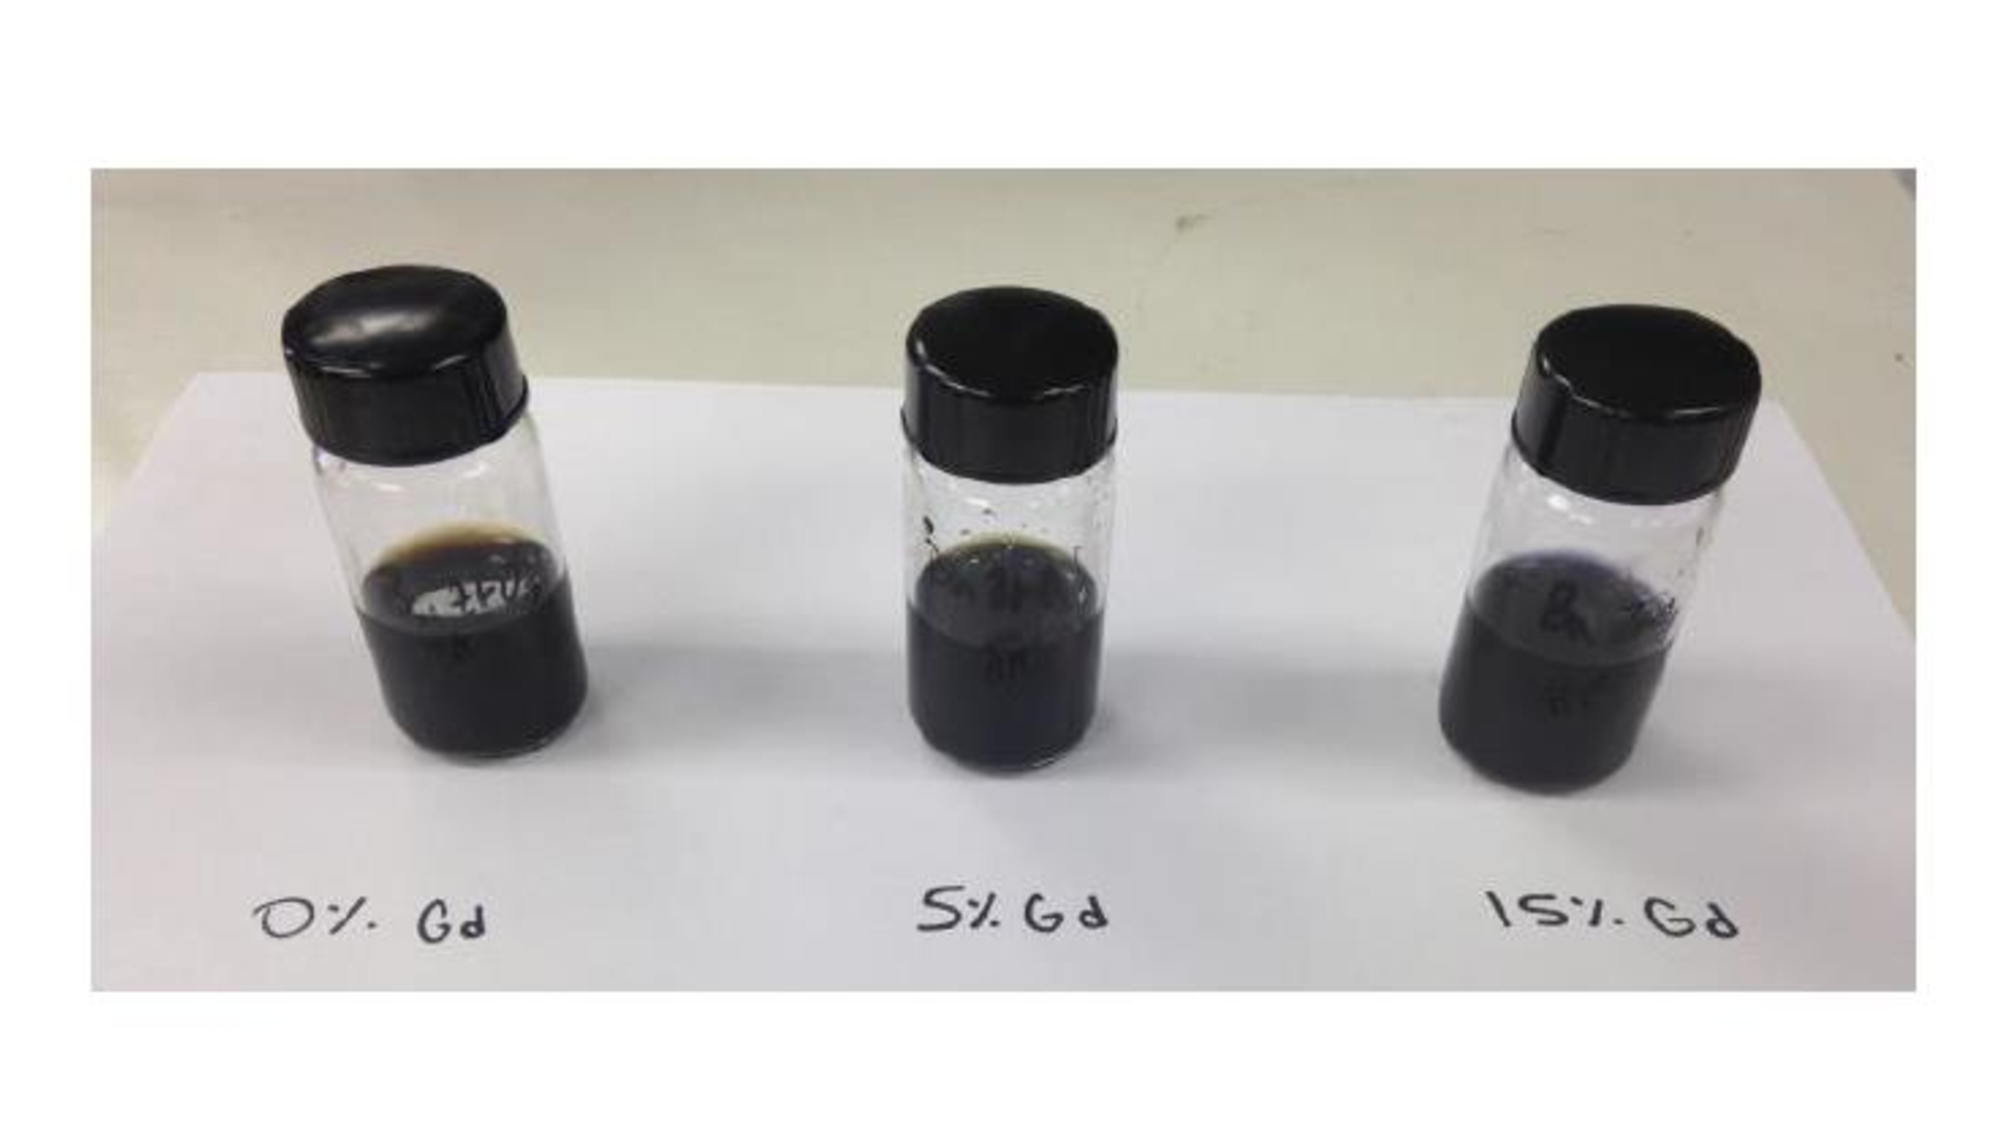
\includegraphics[scale=.35]{Figures/Resin.pdf}
    \caption{Samples after first drying cycle at 100\textdegree C. Water was added to re-suspend the resin. Reproduced from Ref. \cite{GCamata2015} with permission.}
    \label{fig:resin}
\end{figure}

\begin{figure}
    \centering
    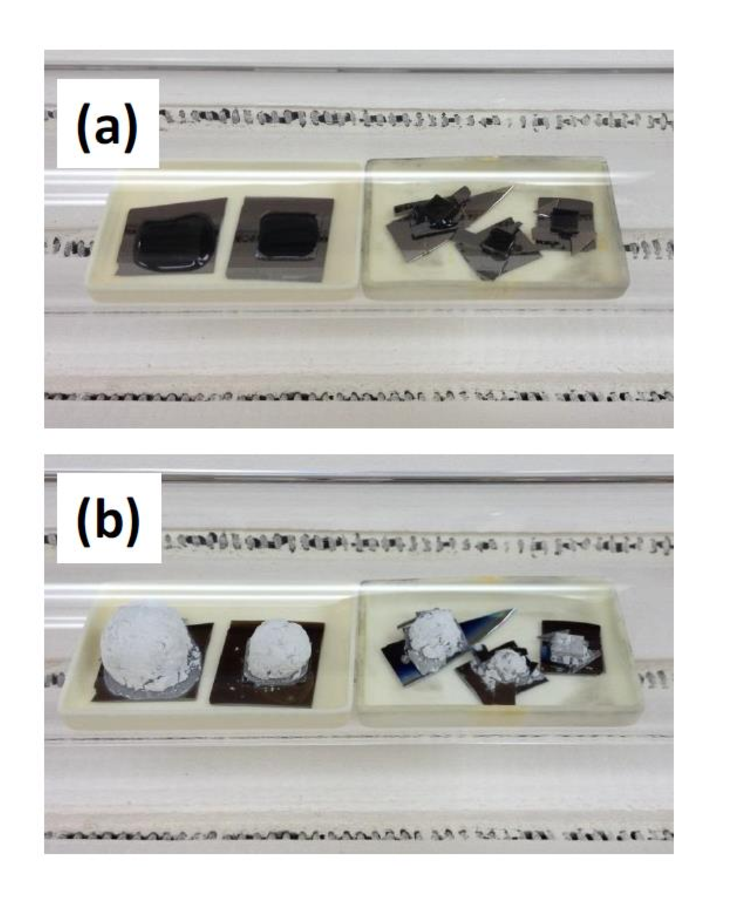
\includegraphics[scale=.75]{Figures/Temp_Treat.pdf}
    \caption{(a) As-dried polymeric resins on silicon substrate (left) and on AlN substrates (right) placed in crucibles inside furnace. (b) Same samples after annealing at 600\textdegree C for 5 hours. Reproduced from Ref. \cite{GCamata2015} with permission.}
    \label{fig:temp:treat}
\end{figure}


This powder was then imaged using scanning electron miscroscopy (SEM) as shown in Figure \ref{fig:chem:sem}, although little can be conclusioned from these images due to the low magnification. However, using the energy dispersive X-ray spectroscopy function of the SEM confirms the presence of gadolinium in the samples, as shown in Figure \ref{fig:chem:edx_1}. This concentration of gadolinium was also confirmed to increase in the larger concentration of gadolinium nitrate added at the precursor stage, showing qualitatively that the gadolinium is preserved throughout the reaction and heat treatment. Figure \ref{fig:chem:edx_2} indicates that the characteristic gadolinium peak at 6.05 keV \cite{Kempen2013} is proportional to the gadolinium added. Compositional analysis from the EDX routine estimate the Gd content of the 5\% sample to be 6.4\% and of the 15\% sample to be 17.3\%. Given the experimental uncertainties inherent with EDX, these are essentially consistent with the dopant concentrations in the chemical preparation. Despite these findings, one cannot ascertain that Gd is in the place of Zr, which is essential for vacancy creation. To determine the exact location of Gd in the material, lattice constant studies, as discussed in the main text for other types of bulk samples, is necessary.


\begin{figure}
    \centering
    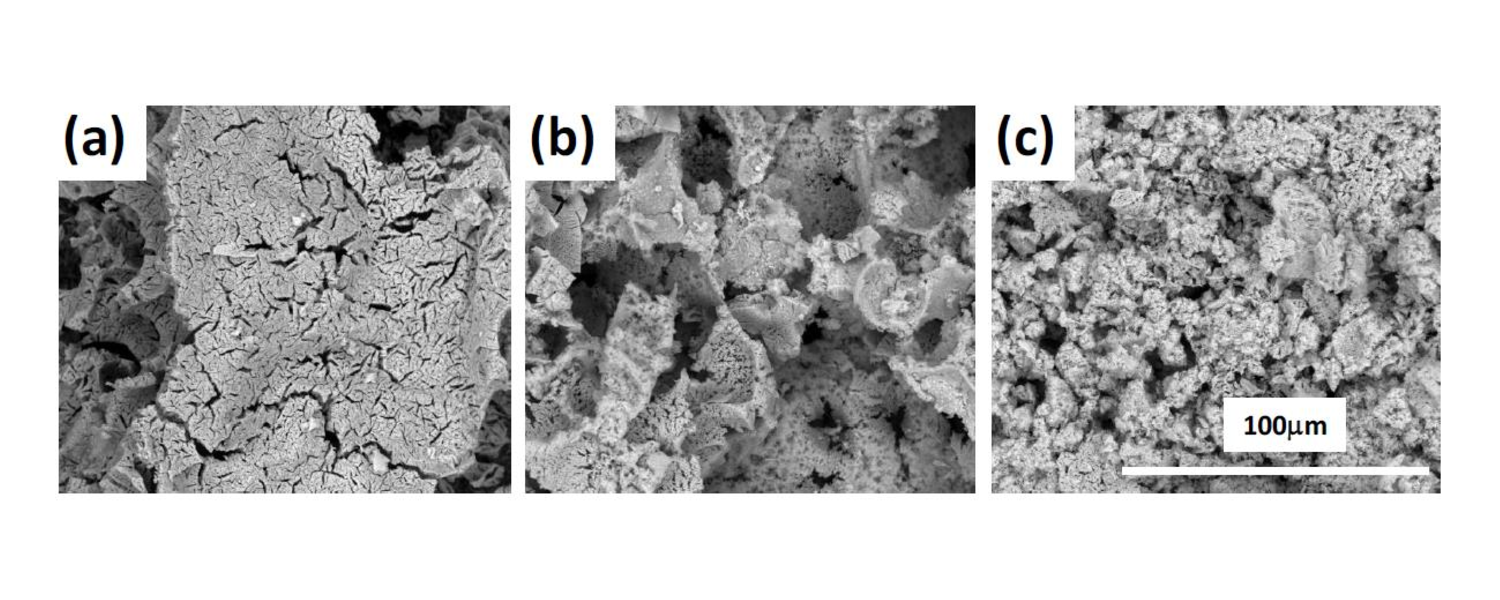
\includegraphics[scale=.50]{Figures/Chem_SEM.pdf}
    \caption{Scanning electron microscopy of (a) pure BaZrO$_3$ sample, (b) 5\% Gd-doped BaZrO$_3$ sample, and (c) 15\% Gd-doped BaZrO$_3$ sample. Reproduced from Ref. \cite{GCamata2015} with permission.}
    \label{fig:chem:sem}
\end{figure}

\begin{figure}
    \centering
    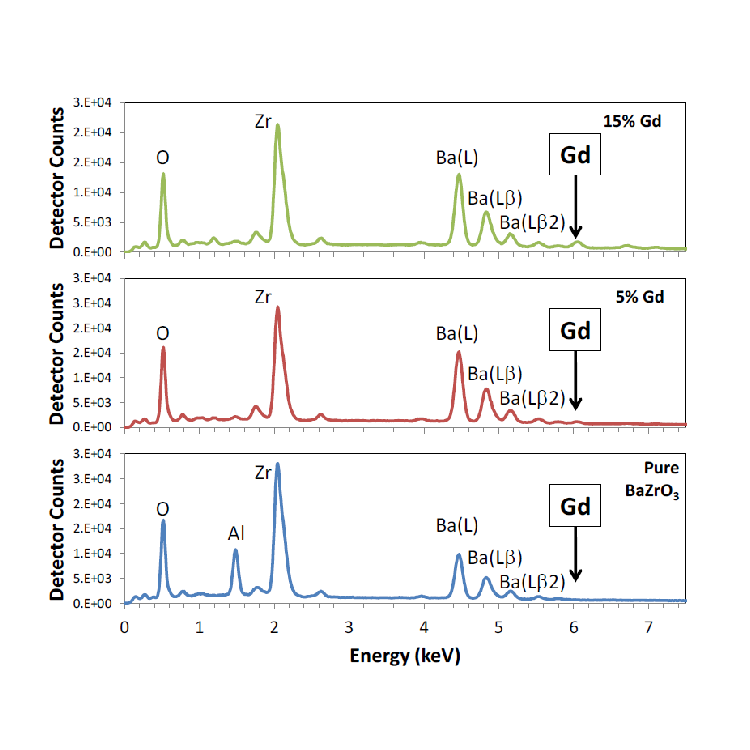
\includegraphics[scale=.75]{Figures/Chem_EDX_1.pdf}
    \caption{EDX spectrum for pure BaZrO$_3$ sample, 5\% Gd sample, and 15\% Gd sample. Peaks correspond to all major constituents of the material. The pure BaZrO$_3$ sample shows an aluminum peak because the sample was dried on an AlN substrate. The 5\% and 15\% Gd samples were dried on Si substrates (Si peak is first to the left of zirconium). Reproduced from Ref. \cite{GCamata2015} with permission.}
    \label{fig:chem:edx_1}
\end{figure}

\begin{figure}
    \centering
    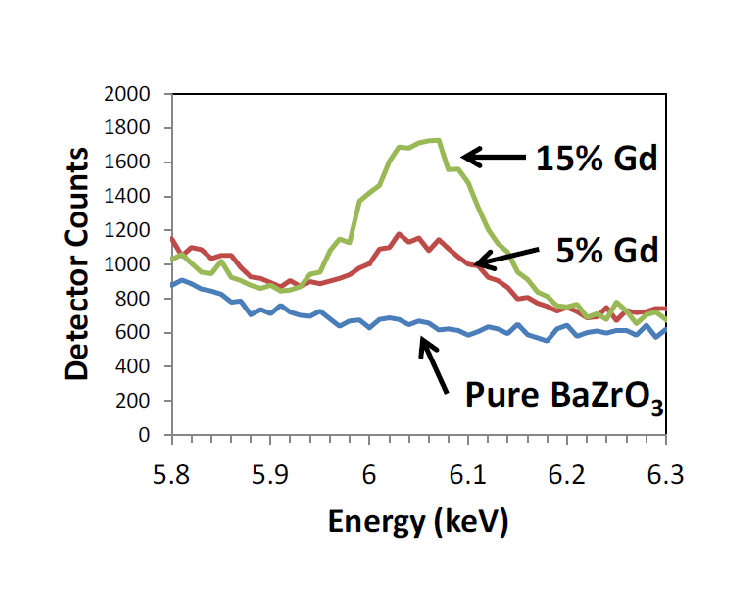
\includegraphics[scale=.75]{Figures/Chem_EDX_2.pdf}
    \caption{EDX spectrum amplifying the Gd peaks. Reproduced from Ref. \cite{GCamata2015} with permission.}
    \label{fig:chem:edx_2}
\end{figure}

Although potentially effective as a bulk material, the powder yield of the process described in this appendix proved to be low and the amount of powder produced in-house by the procedure was unsuitable for pressing the needed pellets. The costs involved in the large amounts of chemical precursors needed and the time-consuming effort to synthesize the tens of grams required for robust bulk samples were impractical. Synthesis using another variation of the Pechini method, known as combustion spray pyrolysis (CSP) was coordinated with a contractor in possession of suitable high-temperature CSP equipment, and used to create a Gd-doped BaZrO$_3$ target of proper dimensions and at a reasonable cost for this project. The CSP method is summarized in the main text of this dissertation.
